\section{PS2: Triangle Fractal}\label{sec:ps2}

\subsection{Discussion}\label{sec:ps2:disc}

For this program, I had to write a program that draws Sierpinski triangle. The input must be depth and length of the triangles. Depth is for the number of smaller trinagles and length is for the length for the first triangle. There should be a big triangle and smaller triangles at its vertices. The positions of small triangles are fixed, so I just had to make a function that draws /2 length of the edges and assign their edges' positions.

\begin{figure}[tbh]
	\centering
	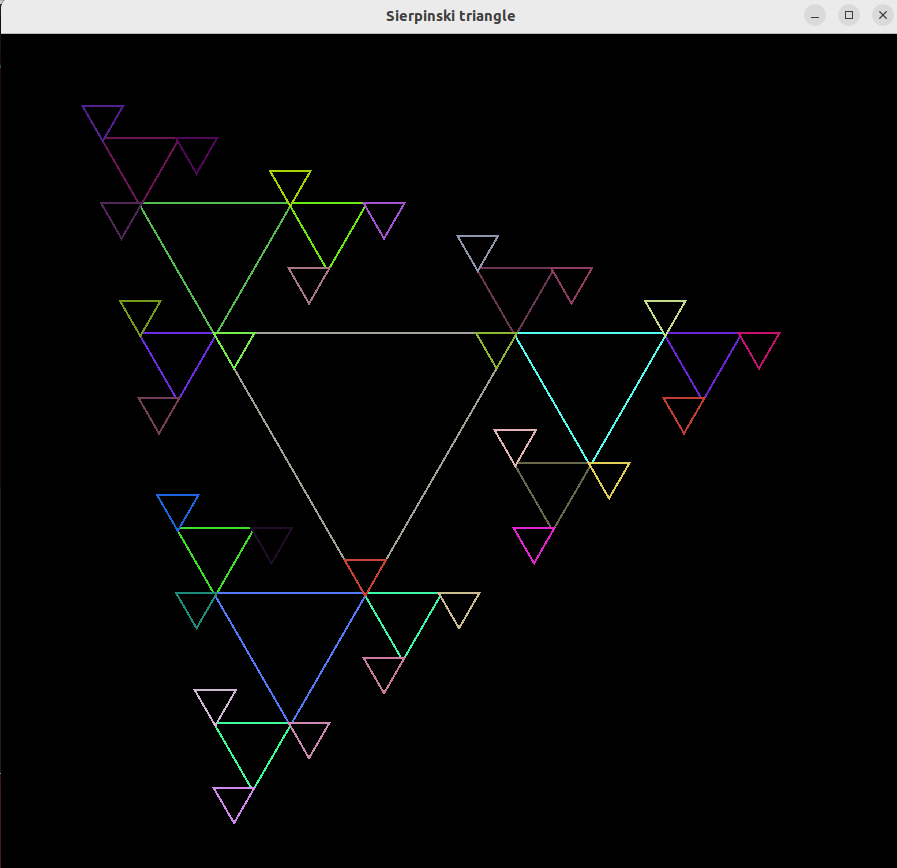
\includegraphics[width=8cm]{triangle}
	\caption{Triangle Fractal with depth of 4 and size of 300}
	\label{fig:Triangles}
\end{figure}


\subsection{Places to get help}
I got help from Samin Patel who helped me to understand what the program is asking for, sfml-dev.org helped me to understand how sf::drawable works.
For coding, c++.com, stackoverflow, and YouTube helped me.

%\subsection{What I accomplished}\label{sec:ps2:accomplish}

%\subsection{What I already knew}\label{sec:ps0:knew}

\subsection{Challenges}\label{sec:ps2:challenges}

I used sf::drawable as a parent inheritance since the project prompt told me to. I tried to make it as a tree only with the class by making other triangles as the members, but it was not working well, so I used vector since c++ has the library for it.

\subsection{Mistakes}\label{sec:ps2:mistakes}

I got two points off because I have one issue with cpplint. I am not sure which code I have to run it with. Whenever I run cpplint code that is provided, it says, "FATAL ERROR: No files were specified." However, I tried to run it with the one on the lectrue note which is ```cpplint *.cpp, *.hpp, it shows many error messages and for some of them which I do not understand what it is asking for.. Also, ironically, it does not check cpp files, so I have to run the code just for cpp again. Since the prompt provided the code, I put that code in my Makefile.

For other point, I did not use command-line parameters instead I used stdin.

\subsection{Extra Credit}\label{sec:ps2:Extra Credit}

The triangles have different colors. I assigned random color code for each triangle's rgb.

\subsection{Codebase}\label{sec:ps2:code}

Makefile
\lstinputlisting[language=Make]{ps2/Makefile}
TFractal.cpp
\lstinputlisting{ps2/TFractal.cpp}
TFractal.hpp
\lstinputlisting{ps2/TFractal.hpp}

\newpage
